\documentclass{article}

\usepackage{graphicx}
\usepackage{mathpazo}
\usepackage{microtype}
\usepackage{parskip}
\usepackage{xpatch}

\usepackage{varioref}
\usepackage[hidelinks]{hyperref}
\usepackage{cleveref}

\newcommand{\navstep}[2]{\navitem{#1}~{#2}~$\rightarrow$}
\newcommand{\navitem}[1]{\textbf{#1}}

\newcommand{\see}[1]{\seewith{see}{#1}}
\newcommand{\See}[1]{\seewith{See}{#1}}
\newcommand{\seewith}[2]{#1 \cref{#2}, ``\nameref{#2},'' \vpageref{#2}}

\newcommand{\encouragebreak}[1]{\vfil\penalty-#1\vfilneg}

\newcommand{\img}[2]{%
  \begin{center}
    \vspace{6pt}
    \encouragebreak{100}
    % use extra \centerline to allow protrusion into margins
    \centerline{\includegraphics[scale=0.5]{img/#1}}
    {\slshape #2}
    \encouragebreak{300}
  \end{center}
}

\xpretocmd{\section}{\clearpage}%
  {}{\typeout{Failed to make sections clearpage!}}
\xpretocmd{\subsection}{\encouragebreak{300}}{}{}

\begin{document}

\begin{titlepage}
  \vspace*{-1in}
  \centerline{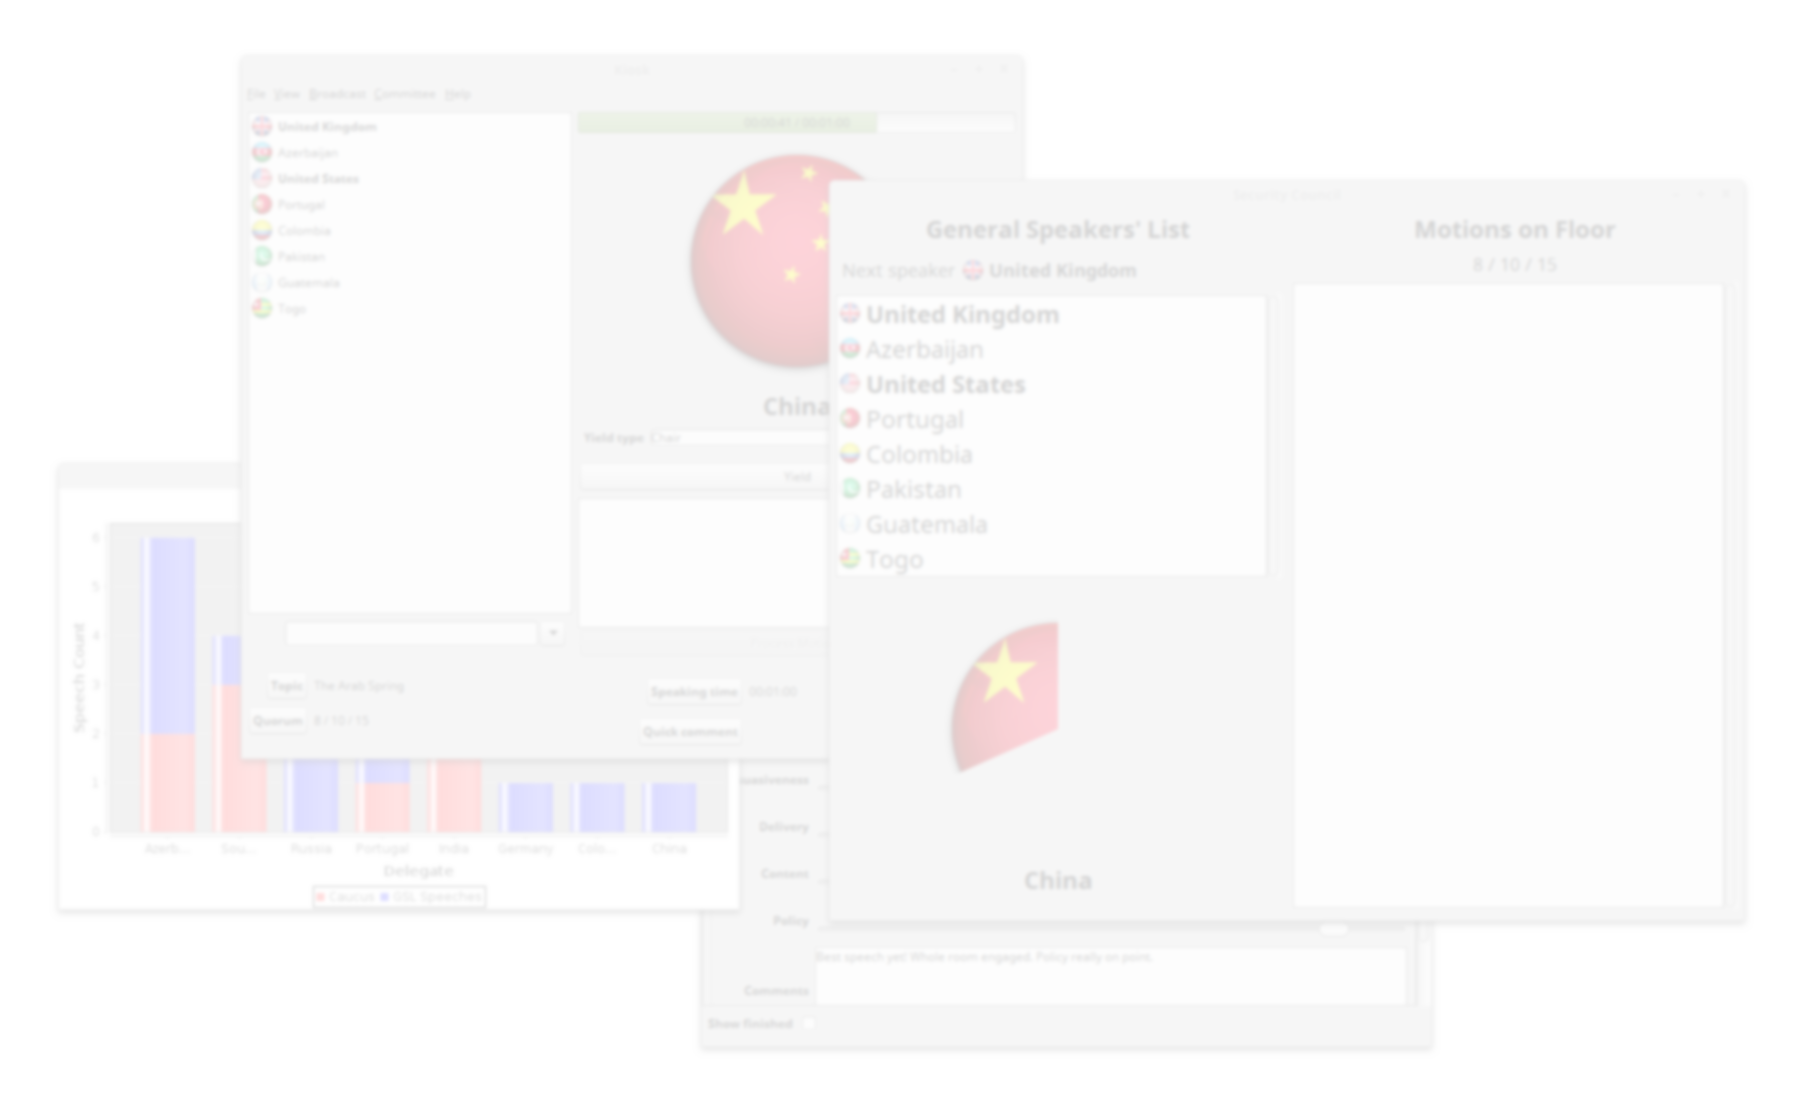
\includegraphics[height=8in]{img/hero_transparent.png}}
  \vspace*{-8in}
  \vspace{3in}
  \centering
  {\Huge \bfseries Kiosk} \\[24pt]
  {\Large User Manual \\[12pt] \itshape for committee directors}
\end{titlepage}

\tableofcontents

\section{Setup}

\subsection{The setup wizard}

When you first open Kiosk, the committee creation wizard will guide you through the process of creating a committee.
You can simply follow the steps in that wizard to create your committee, and then skip to the section ``Quorum''~below to take roll.
If you prefer not to use the wizard, read on to learn how to manually set up the committee.

\subsection{General committee setup}

The first thing you need to do to prepare for a committee is to define the basic committee information.
In particular, you must define the committee's name and the list of topics on the agenda.
You can also change the default speaking time or the number or duration of allowed comments.
All these settings appear under \navstep{Committee}{menu} \navitem{Configure Committee}.

\img{configure_committee}{The ``Configure Committee'' dialog.}

\subsection{Delegate setup}

Once you've set up your committee, you'll also need to define its members.
You can manage delegates by clicking \navstep{Committee}{menu} \navitem{Manage delegates}.
Enter the name of a delegate in the text box, and press~Enter or click~``Add'' to add the delegate.

\img{manage_delegates}{The ``Manage Delegates'' dialog.}

You can also double-click any delegate to access more advanced settings---for example, to grant the delegate veto power in the security council, or to change the delegate's icon.
(Delegates representing countries are automatically given the corresponding flag icons.)

\img{manage_delegates_grant_veto}{Editing specific properties of a delegate.}

\subsection{Quorum}

Once you've set up all delegates in your committee, you're ready to start debate as soon as you establish quorum.
To do so, click \navstep{Committee}{menu} \navitem{Quorum}, or click the \navitem{Quorum} button at the bottom of the window.
Mark each delegate as absent, present (the default), or present and voting, as the case may be.

You should re-establish quorum each time the committee enters session.

\section{The general speakers' list}

To add delegates to the General Speakers' List, enter the delegate's name into the text box at the bottom.

To start a speech, double-click the delegate's name in the speakers' list.

If a delegate finishes a speech early, you can double-click on the delegate's name or flag to stop the speech.
To pause a speech, click only once.
To yield to comments, questions, or another delegate, select the appropriate yield type from the \navitem{Yield type}~dropdown under the speaker, and then click \navitem{Yield}.

\img{general_speakers_list}{%
  A typical view in the general speakers' list, with an ongoing speech, some queued speakers, and a delegate (Russia) being added to the queue (in the bottom left).
}

\section{Motions}

\subsection{General}

All motions are proposed from the \navitem{Committee}~menu.
For example, if a delegate motions for a moderated caucus, select \navstep{Committee}{menu} \navstep{Caucus}{submenu} \navitem{Moderated Caucus}, or press the shortcut key listed there.
This will bring up the caucus configuration dialog.

\img{moderated_caucus_configuration}{An example motion, configuring a moderated caucus.}

When there are any motions on the floor, you should collect all proposed motions from delegates before voting on any.
Then, once all motions have been recorded, click \navstep{Committee}{menu} \navitem{Process Motions on Floor}, or click the \navitem{Process Motions}~button beneath the list of motions.
This will automatically sort the motions in the correct order (from most to least disruptive), and then begin voting on the most disruptive motion.

\img{motions_on_floor}{The ``motions on the floor'' panel after two motions have been proposed; click the button here to begin the voting process.}

Once the voting dialog appears, you should count the votes and determine whether the motion has passed.
(Note that the quorum indicator in the main panel indicates how many votes are needed to pass: a line reading ``Quorum: 8~/~10~/~15,'' for example, indicates that there are 15~members present, so the requirement for simple-majority motions is 8~votes and the requirement for two-thirds-majority motions is 10~votes.)
Then, select the appropriate action from the drop-down menu.
At this time, you can also rule a motion as dilatory, or, conversely, unilaterally approve it.
\img{vote_on_motion}{The voting dialog that appears for a motion under consideration.}

If a motion passes, all other motions on the floor will be removed.
If a motion fails, voting will proceed to the next motion.

\subsection{Debate on motions}

Some motions, as a Motion to Set the Agenda, allow two speakers in favor of the motion and two speakers against, while other motions, such as a Motion to Close Debate, allow only two speakers against.
If either such motion comes to a vote, a speakers panel will appear.
If a delegate wishes to speak, double-click that delegate's name and the timer will begin.
As usual, double-click the flag or name to end the speech early.

\img{speak_for_motion}{A delegate speaking in favor of a motion to set the agenda.}

When both speakers for each side have spoken, voting will commence on the motion.
If no one wants to speak, you can click ``Close'' to skip the speaking phase.

\section{Caucuses}

Conduct in caucuses is slightly different from conduct on the General Speakers' List.
The exact differences depend on the type of caucus.

\subsection{Moderated caucus}

Within a moderated caucus, the speakers' list will be hidden, and a list of all present delegates will appear on the left.
Select a delegate from this list to recognize that delegate.

\img{moderated_caucus}{A typical moderated caucus view, with a delegate giving a speech.}

The upper time bar represents the time remaining in the moderated caucus.
The lower time bar represents the time remaining for the current speech.
If there are no delegates wishing to speak, you may end the caucus early by selecting \navstep{Committee}{menu} \navstep{Caucus}{submenu} \navitem{Return}.

\subsection{Formal caucus}

To propose a formal caucus, you must first introduce a working paper (\see{sec:wpdr}).
When proposing the motion, select the relevant working paper in the motion configuration dialog.
\img{formal_caucus_proposal}{Proposing a motion for a formal caucus, accompanied by a working paper.}

In a formal caucus, sponsors or signatories of the working paper or draft resolution approach the podium, have the option to read the document, and answer questions in a lightly moderated format.
If the public display is open, delegates will see the document projected (\see{sec:public-display}).
\img{formal_caucus_public_view}{A formal caucus in progress, as shown to delegates in the public panel.}

\subsection{Unmoderated caucus}

In an unmoderated caucus, the speakers' list will be replaced with a progress bar indicating how much time remains in the caucus.

\section{Working papers and draft resolutions}
\label{sec:wpdr}

\subsection{Introducing working papers and draft resolutions}

If a delegate motions to introduce a working paper, select \navstep{Committee}{menu} \navstep{Other Motions}{submenu} \navitem{Motion to Introduce Working Paper}.
If the motion passes, you will see the working paper setup dialog.
If the delegate is using Google Docs, you should ask them for the document ID of their document and input that in the ``Google Docs ID'' field; otherwise, you should ask them to send you a PDF, and attach that PDF to the working paper.
(Using Google Docs is preferred because the documents can update automatically.)

You can also unilaterally introduce a working paper, without a motion, by selecting \navstep{Committee}{menu} \navstep{Working Papers and Resolutions}{submenu} \navitem{Introduce Working Paper}.
From the same menu, you can promote a working paper to a draft resolution by selecting \navitem{Introduce Draft Resolution}, or edit existing working papers or draft resolutions---for example, to change sponsors or signatories---by selecting \navitem{View and~Edit}.

\img{editing_working_papers}{Editing a working paper.}
\img{editing_draft_resolution}{Editing the above working paper after its promotion to a draft resolution.}

\subsection{Voting}

To vote on a draft resolution, select \navstep{Committee}{menu} \navitem{Substantive Vote}.
From the dialog that appears, you may either count votes as usual, or unilaterally entertain a roll call vote (also accessible under the \navitem{Other Motions}~submenu of the \navitem{Committee}~menu).
If manually tallying votes, make sure to select the ``Vetoed''~checkbox if a delegate with veto power votes ``no.''

\img{substantive_vote_manual}{Manually tallying votes for a substantive vote.}

If you select ``Roll Call Vote,'' or a Motion for Roll Call Vote passes, you will be prompted to select each delegate's vote.
Veto members' ``No'' and ``No with rights'' options will read ``Veto'' and ``Veto with rights,'' respectively.

\img{substantive_vote_roll_call}{Proceeding through delegates in a roll call vote.}

At the end of voting, any delegates who elected to vote with rights will be given 30~seconds to speak.

\img{substantive_vote_with_rights}{A delegate exercising their right to speak after the votes have been tallied.}

Finally, when the voting and speaking have completed, the voting result will appear.

\img{substantive_vote_result}{The result of the vote, indicating the totals and the veto status.}

\section{Crises}
\label{sec:crises}

Many committees make use of \emph{crises}: real-time updates engineered to drive the debate in a certain direction, or to prevent the debate from stagnating.
To set up crises for your committee, select \navstep{View}{menu} \navitem{View crises}.
Click the \navitem{Add crisis}~button to add your first crisis, then click~\navitem{Edit} to edit it.

\img{crisis_configuration}{Configuring the crisis.}

When you click~\navitem{OK}, the entry in the list of crises will update.

\img{crisis_list}{The updated crisis list after making the changes shown in the previous figure.}

The red bar indicates that the crisis has not yet been deployed. After you deploy the crisis, the bar will turn green.

To deploy the crisis, click the \navitem{Display}~button.
The public display, if open, will switch to Crisis Mode.
In crisis mode, the attached crisis briefing (if any) will be displayed, as well as information about the guest speaker (if any) and Q\&A~session (if any).

If you select a guest speaker, the speaker may give a statement for as long as they wish.
If you additionally select a Q\&A~session, you will have the option to start the session whenever the speaker finishes their statement.
You cannot have a Q\&A~session without a guest speaker.

Throughout the whole crisis, the briefing (likely a fake news article) will be displayed in the public display.

\img{crisis_ongoing}{The crisis as it appears in the public display, with a timer for the Q\&A~session at the bottom.}

In the main Kiosk screen, a dialog with the crisis file will also appear.
If you have selected a Q\&A~session, click \navitem{Start Q\&A~Session} once the guest speaker has concluded their statement to start the timer.
Closing this dialog will conclude the crisis.

\section{Public display}
\label{sec:public-display}

If you connect your computer to a projector, you probably don't want all the delegates to see everything you can see: it's more information than they need, and it could give them privileged information about future crises.
Instead, open the public display by selecting \navstep{View}{menu} \navitem{Show Public Display}.

Then, configure your machine to project just this window\ldots
\begin{description}
  \item[for Windows]
    opt to ``Extend'' your desktop by pressing \navitem{Start key}-\navitem{P} on Windows~7 or higher, or opening the Windows Mobility Center control panel on older versions;
  \item[for Mac~OS or most Linux distributions]
    turn off ``mirroring'' in the \navitem{Displays} system preference pane.
\end{description}

The public display provides delegates with exactly the information they need to work most productively in committee session.
The display runs completely automatically, and requires no configuration or control on your part.

The display has seven main modes:
\begin{description}
  \item[General Speakers' List]
    This view is shown whenever the speakers' list is active.
    It contains a copy of the speakers' list; if the list overflows, it will automatically scroll through the speakers repeatedly.
    If a delegate is speaking, the view shows the delegate's icon and indicates how much time remains.
    The view also contains a list of any motions on the floor.
    \img{public_panel_gsl}{%
      A sample view of the public display on the general speakers' list.
      At this time, the delegate of Morocco~is speaking, and about~40\% of the time allotted to Morocco's speech has elapsed (as indicated by the circular flag icon).
      The list of speakers is automatically scrolling, and is near the bottom.
      For demonstration purposes, a motion is on the floor (although speeches and motions don't occur concurrently in a real debate).
    }
    \img{public_panel_yield_to_delegate}{%
      This excerpt from the public panel shows the view when a delegate (China) yields the remaining time to another delegate (Russia).
      In this example, China used about a sixth of the initial time, and Russia has used almost half of the remaining time.
    }
  \item[Moderated caucus]
    In a moderated caucus, the view shows the purpose of the caucus, as well as a timer indicating how much time remains in the caucus and how much time the current speaker (if any) has left.
  \item[Unmoderated caucus]
    The unmoderated caucus view simply shows a progress bar indicating how much time remains.
  \item[Formal caucus]
    The formal caucus view contains a copy of the working paper or draft resolution being discussed.
    It also shows the amount of time remaining in the caucus.
  \item[Crisis]
    During a crisis, the crisis briefing is always displayed.
    The guest speaker's name and role are listed, if there is a guest speaker.
    The status of any Q\&A~session (whether it has started and, if so, the time remaining) is also displayed.
    \See{sec:crises} for more information.
  \item[Voting bloc]
    When a substantive vote is in progress, the public display will automatically enter voting bloc mode.
    In voting bloc mode, no content is displayed; instead, a message asks staff to seal the chamber doors and delegates to suspend note passing.
  \item[Working paper viewer]
    This optional mode can be activated manually, and displays any working paper or draft resolution that you choose.
    Select \navstep{View}{menu} \navitem{View WPs/Draft Resolutions} to activate it.
\end{description}

\section{Networking}

Using Kiosk on the network grants you access to three key features: the broadcast system, the speech analysis system, and OmniKiosk.
To enable networking, select \navstep{Broadcast}{menu} \navitem{Start Server}.
You can find your IP~address by clicking \navstep{Broadcast}{menu} \navitem{Server Info}.
The following sections assume that you have started the server and know your IP~address.

\subsection{Broadcast system}

Assistant chairs can use the broadcast system to receive a continuous stream of updates on committee events, such as when a delegate has ten seconds remaining or a caucus has ended.

Open the Receiver companion application and enter the IP~address of the main Kiosk.
Messages will arrive as events occur.

\subsection{Speech analysis}

With the speech analyzer, you can keep track of every GSL and moderated caucus speech, and analyze them pursuant to four key criteria: content, delivery, persuasiveness, and adherence to policy.

Check the ``Completed'' box once you complete each analysis; the speech will then be hidden unless you check ``Show completed'' at the bottom.

\img{analyzer_edit}{A rapporteur taking notes on a speech.}

To see real-time graphs of speech statistics, click \navstep{View}{menu} \navitem{Speech Graph}.
Delegates will be sorted by greatest number of speeches.
Hover a bar section to see exactly what it represents.

\img{analyzer_graph}{%
  The live speech graph for a debate. 
  The bar under the mouse cursor indicates that Azerbaijan has spoken three times in moderated caucuses.
}

You can save your speech analyses into a Speech Analysis Index (\texttt{.sai}) file.
At the end of the conference, you can export either the delegate averages or each individual speech entry to a Comma-Separated Values (\texttt{.csv}) file that can be read by most spreadsheet applications, including Excel, Numbers, Calc, and Google Docs.
Select \navstep{File}{menu} \navitem{Export to CSV}.

\subsection{OmniKiosk}

OmniKiosk is a service for conference organizers that allows overseeing all Kiosks on the network.
By starting the broadcast server, you allow an OmniKiosk on the network to discover you.
You can have one-way communication with the OmniKiosk by clicking the \navitem{Quick comment}~button in the Kiosk.
The OmniKiosk user (likely the Secretary-General) can see any comments you enter here, as well as other information about your committee.

\img{omnikiosk}{%
  A sample OmniKiosk.
  Note that OmniKiosk works across operating systems (shown here: a Windows~7 OmniKiosk with host Kiosks on Linux and~Mac).
}

In particular, the OmniKiosk user can see:
\begin{description}
  \item[Committee status]
    In the example above, DISEC is in an unmoderated caucus, and the Security Council is in a moderated caucus.
    Other statuses and icons include the General Speakers' List (a single speech bubble), Formal Caucus (a piece of paper), and Voting Bloc (a check mark).
  \item[Current topic]
    The current topic of a committee is displayed directly below its name.
  \item[Working papers and draft resolutions]
    The number of working papers and draft resolutions is displayed in a circle: in the example, DISEC has no such papers, and the Security Council has a total of two.
  \item[Comments from chairs]
    Any comments entered in the \navitem{Quick comment} section of a Kiosk appear below the current topic.
  \item[Last check-in time]
    Kiosks check in every five seconds; due to network lag or spotty connections, the time to receive may be up to thirty seconds.
    When more than thirty seconds have passed, it is likely that the Kiosk has been closed.
\end{description}

\section{Tips and tricks}

The following tips and tricks may be helpful for chairs and conference staff!

\begin{description}
  \item[Set your committee to autosave]
    To make your committee automatically save after a certain period of time (by default, ten minutes), select \navstep{File}{menu} \navitem{Autosave\ldots}.
  \item[Make use of the Document Viewer]
    At any time, you can override the content of the public display, replacing it with any given working paper or draft resolution.
    This is frequently valuable, helping delegates reference the latest version of pertinent information without needing individual laptops.
    Select \navstep{View}{menu} \navitem{View WPs/draft resolutions}; when done, select \navstep{View}{menu} \navitem{Standard debate} to return to the normal view.
  \item[Try using Dropbox or a similar service]
    If you're not the only chair in your committee, consider setting up a shared Dropbox account.
    This will let you synchronize files across computers: whenever you save a file on one computer, it will be updated on the others.
    In particular, you can share a folder for your committee with your co-chairs, including your committee session (\texttt{.mun}~file), speech analyses (\texttt{.sai}~file), and any other committee-related materials, such as working papers.
    This allows any chair to take over for any other without needing to share a computer.
  \item[Send a message to your unruly delegates]
    If your committee is starting to get out of control, click \navstep{View}{menu} \navitem{Flash: ``Decorum''} to display a very visible warning across the public panel!
\end{description}

\section{Support, feedback, and contact information}

\def\emailtld{com}
\def\emaildomain{gmail}
\def\emailuser{wchargin}
You can reach me at \texttt{\emailuser@\emaildomain.\emailtld}---and please do feel free to reach out with any feedback!

If you need help using Kiosk, please let me know the version of Kiosk you're using and your Java version.
You can find both of these in the \navstep{Help}{menu} \navitem{About}~dialog within Kiosk.

\img{version_info}{%
  The version info dialog: the Kiosk version here is~3.3, and the Java version is~1.8.0\_66.
  Please send these numbers to me if you have a technical problem.
}

I~owe a hearty thanks to Brad Ross, who gave me design advice and a plethora of suggestions along the course of making this program.
Furthermore, this program would not be possible without the support of the dozens of chairs who've consistently given me valuable feedback.
Finally, I~want to thank the League of~Creative Minds for allowing me to test this software at their conferences.
It's been a blast!

\end{document}
